% Chapter Template

\chapter{Implementation} % Main chapter title

\label{Chapter5} % Change X to a consecutive number; for referencing this chapter elsewhere, use \ref{ChapterX}

%----------------------------------------------------------------------------------------
%	SECTION 1
%----------------------------------------------------------------------------------------

\section{Inputs and outputs}

As any other React component you can simply import the main class into your current project and that's pretty much all. Then you can customize the component, provide it some data and start using it. Detailed API is in the appendix, there you can find all properties that you can use. 

The most important property is 'options', this property represents actual options that will be rendered. These options can be represented in two ways. As a graph (simplified version) where each node is represented as one object or as a list of objects (non-simplified) where children are parts of the parent. You can see an example of the options structure in the figure \ref{fig:input-data-example} down below.

Another important property is 'onInputChange', this is a function that will be called when a user selects an option. So this is the way how you can get all selected options. The option that you get back will not be same as you provide. The structure of the new option is following:
\begin{center}
    \begin{longtable}{ | l | l | p{10cm} | }
    \caption{Structure of the returned option} \label{tab:perf} \\
    \hline 
    \multicolumn{1}{|c|}{\textbf{Key name}} & 
    \multicolumn{1}{c|}{\textbf{Type}} & 
    \multicolumn{1}{c|}{\textbf{Description}} \\ \hline 
	\endfirsthead
    \hline 

	provider & Object & object representing provider of that option. See appendix for more detail structure of this object \\ \hline
    state & Object & Object representing state of the option. E.g. \{label: 'Merged', color: 'warning', message: '...'\}, \\ \hline
    expanded & Boolean & Represent if option is expanded (children should be rendered or not)\\ \hline					
    'childrenKey' & List & List of the children IDs. Key name stay same as childrenKey value\\ \hline
    ... &  &  All other properties that was in the original object\\ \hline
    

    \end{longtable}
\end{center}
 

%----------------------------------------------------------------------------------------
%	SECTION 2
%----------------------------------------------------------------------------------------

\section{Component parts}

%----------------------------------------------------------------------------------------
%	SUBSECTION 2.1
%----------------------------------------------------------------------------------------
 \subsection{Virtualized-tree-select part}

Main part virtualized-tree-select component is custom component build on react-virtualized-select and react-select.
This component retains the same API as both components, in addition it provide several new configurations, that configurations can be seen in appendix. So as React-Select, this component generates hidden text input field that contains the value of the
selected option, so it could be submitted as part of the standard form. When the option is selected, ‘onChange’ event is
fired and this event return selected option. All the changes to the select input must be handled by the user; the user
must pass that event value to the ‘value’ attribute of the select component.


%----------------------------------------------------------------------------------------
%	SUBSECTION 2.2
%----------------------------------------------------------------------------------------

\subsection{Settings part}

This is just a collapsible form with several checkboxes that provide some changes to the Virtualized-tree-select
component, like expand or collapse all. Multi-select, this option, if it is checked then the component will provide
multi-selection otherwise only one option will be selectable. Render as a tree, as the name suggests, this option
renders all nodes as a tree also it slightly change filtering because by default if this option is checked the filtering
will also show the whole path in the tree, meaning all parents until root parent will be displayed as well. Display info
on hover, this option enables to show additional information for that node on hover. For example, description.

\begin{figure}[th]
    \centering
    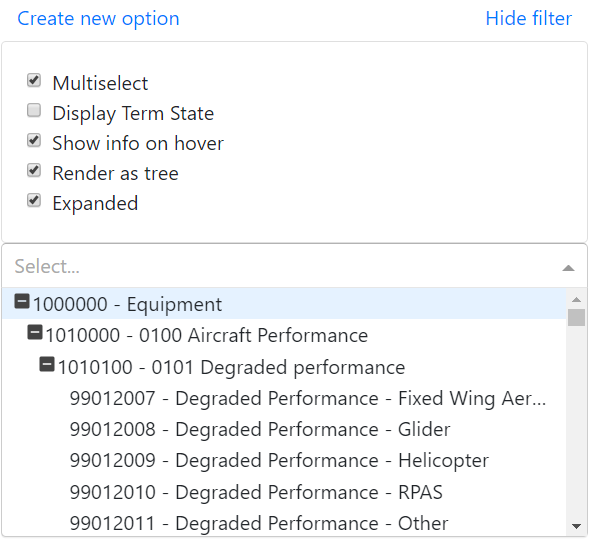
\includegraphics[width=\textwidth]{its-component}
    \decoRule
    \caption[Intelligent tree select component]{Virtualized tree select component with expanded settings}
    \label{fig:its-component}
 \end{figure}

%----------------------------------------------------------------------------------------
%	SUBSECTION 2.3
%----------------------------------------------------------------------------------------
\pagebreak

\subsection{Modal form part}

This component part consists of two dependent react classes. The first one renders empty modal dialog that contains an
only header and close button. The second one renders the actual redux-form in modal body and actions buttons for
submitting or canceling in the modal footer. As I mentioned earlier, this redux-form is used for creating new Nodes. It has several form fields:
\begin{itemize}
    \item Option label (required) – representing a value that is visible in a drop-down box
    \item Option value (required) – representing the unique ID
    \item Option description
    \item Children – a multi-select box containing labels of all other options
    \item Parent – select box containing labels of all other options
\end{itemize}
In the advanced section, there is a button that adds a new pair of form fields. The first one represents object key, second one object value.


After each key press validation is triggered, so the user is informed about invalid inputs before submitting that form. Also, the form is submitted only in the case when all fields are valid. After that new node is created and its added to current tree graph and event ‘onNewOptionCreation’ will be fired.

\begin{figure}[th]
    \centering
    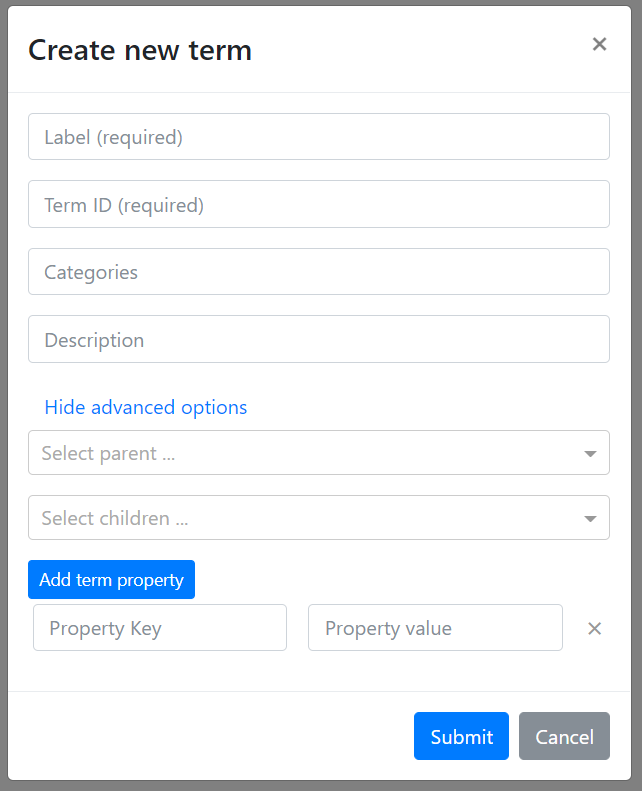
\includegraphics[width=0.7\textwidth]{redux-form}
    \decoRule
    \caption[Redux form]{Redux form for adding new terms}
    \label{fig:redux-form}
 \end{figure}

%----------------------------------------------------------------------------------------
%	SECTION 3
%----------------------------------------------------------------------------------------



%----------------------------------------------------------------------------------------
%	SECTION 4
%----------------------------------------------------------------------------------------

\section{Performance}

Usability of the application may be affected by the performance of the used components. So the performance of my component was one of the critical points during the development. Even that the performance of the current version is acceptable, I still think that there is a space for improvements so that I will continue with the research in this field. As you may know for the flexibility, you have to pay something. Several algorithms have an impact on the overall performance. These algorithms are:

\begin{enumerate}
\item Filter algorithm
\item Algorithm responsible for rendering drop-down menu with options
\item Algorithm that merge all duplicate options
\item Sort algorithm
\item Algorithm for processing data
\end{enumerate}

%----------------------------------------------------------------------------------------
%	SUBSECTION 4.1
%----------------------------------------------------------------------------------------
\section{Render algorithm}

These, who have good experience with HTML, may know that rendering process is a lengthy operation, compared to the JavaScript computation. So I decided to include \cite{react-virtualized-select} that can perfectly handle the problem with rendering a large number of options. The first method is menu rendered and the second one is row renderer. Row renderer is responsible for rendering individual options. Menu renderer renders drop-down menu. This method takes several parameters, most important are - filtered options, currently focused option, option height, drop-down menu height. From these parameters, it can compute how many and what options should be rendered and call row renderer for each of these options. 

The best way is to provide an example. Let's say that filtered options is an array of 20 options. Currently focused option has an index equal to 10. Option height is 20px (pixels) and dropdown height is 100px. So the algorithm renders a container representing dropdown menu with 100px height, then the empty container with a height equal to 400px (20 options times 20px each option) into that previous container. Then algorithm renders individual options with the specified offset, so the method that renders each option is called for the ninth to sixteenth options.

%----------------------------------------------------------------------------------------
%	SUBSECTION 4.2
%----------------------------------------------------------------------------------------
\subsection{Filter algorithm}

The second algorithm that affects performance is an algorithm that filters all options. This algorithm can be divided into three parts. First, all matching options are filtered out. Second, for each filtered option find all parent options (this part will be conditional in future). Last part, all options that are not expanded (their parent have expanded set to false) are also filtered out. 

In detail, the method for filtering options takes 3 arguments. All options, match string and selected options. First of all, options that contain a match string are filtered out. Then the parent options are found for each filtered option. Finding a parent option is done a constant time because the internal data structure of options is same as the structure that is used by Firebase real-time database \parencite{firebase}, which is JSON tree structure. I choose this structure because data are represented as one big JSON object where keys correspond the option value (unique ID of that option) and values of the JSON object are options itself. This structure enables to access the options in constant time. And finally, the algorithm for every option of that previous sub-process (finding parents),  check if an option has a property called 'expanded' equal to 'true', if not then the algorithm removes all children options of that option.

%----------------------------------------------------------------------------------------
%	SUBSECTION 4.3
%----------------------------------------------------------------------------------------
\subsection{Merge algorithm}

Next algorithm merges all duplicate options based on the provider's priority. This algorithm is executed only when new options are added. So if you decided to use only VirtualizedTreeSelect component where you include all options directly this algorithm is never executed. Anyway, this algorithm for each new option checks if that option is already present in the array of all cashed options. If no, then simply adds it and if yes then updates it.

%----------------------------------------------------------------------------------------
%	SUBSECTION 4.4
%----------------------------------------------------------------------------------------
\subsection{Sort algorithm}

Sort algorithm is included in the method that processes all input data. Like the previous algorithm, this algorithm is executed when new options are added. This process takes the option and adds some keys that are used, e.g., parent ID, expanded, state and depth. This algorithm has the same approach like a depth-first search algorithm \parencite{dfs}. So the first item in that sorted array is a root node, next item is left children node of that node and so on, and the last item in last right leaf node.


%----------------------------------------------------------------------------------------
%	SUBSECTION 4.5
%----------------------------------------------------------------------------------------
\subsection{Performance results}

Now let's look at some numbers and data. In this table below you can see how long does is to take for each process to finish. 
For the test purpose, I have one large dataset of 2617 options represented as a graph (simplified) \ref{fig:simplified-data-example} and one smaller dataset of 480 options represented as an array of objects with children as their properties (non-simplified) \ref{fig:non-simplified-data-example}. 

These datasets represented types of aviation accidents and were provided by the \groupname (KBSS). Usage of these datasets is in the INBAS (https://www.inbas.cz/reporting-tool) project. Actual test data will be provided together with the source code.

\begin{figure}
  \centering
  \begin{subfigure}{.5\textwidth}
    \centering
    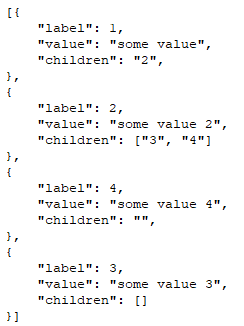
\includegraphics[width=\textwidth]{simplified-data-example}
    \caption[Simplified dataset]{Example of simplified data structure}
    \label{fig:simplified-data-example}
  \end{subfigure}%
  \begin{subfigure}{.5\textwidth}
    \centering
    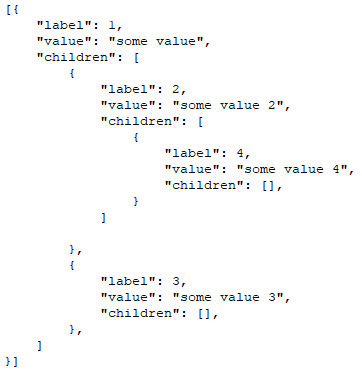
\includegraphics[width=\textwidth]{non-simplified-data-example}
     \caption[Non-Simplified dataset]{Example of non-simplified data structure}
    \label{fig:non-simplified-data-example}
  \end{subfigure}
  \caption[Input data example]{Example of data structure}
  \label{fig:input-data-example}
\end{figure}



This table represents the tests results. Each test was done 10 times on two different test machines and two different web browsers. Data in the table are average values.

\begin{center}
    \begin{longtable}{ | l | l | l | }
    \caption{Time performance based on data structure and data size} \label{tab:perf} \\
    \hline 
    \multicolumn{1}{|c|}{\textbf{Method}} & 
    \multicolumn{1}{c|}{\textbf{Data type}} & 
    \multicolumn{1}{c|}{\textbf{ $\sim$ Time to finish}} 
	\endfirsthead
    
    \hline 
    
    Add new options & simplified & 90 - 200 ms \\ \hline
    Process options & simplified & 4-7 ms \\ \hline
    Filter options & simplified & 1-7 ms \\ \hline
    
    Add new options & non-simplified & 3-5 ms \\ \hline
    Process options & non-simplified & 0-1 ms \\ \hline
    Filter options & non-simplified & 0-1 ms \\ \hline
    Convert dataset & non-simplified & 3-4 ms \\ \hline

    \end{longtable}
\end{center}

Tests were done on two PCs and on the different browsers. However, the differences are negligible (0-2 ms). 
\bigskip

The first test machine specification: Intel i7 series 2.8 Ghz, 16GB ram, win10.
Second test machine specification: AMD FX series 3.5Ghz, 8GB ram, win10. 
Both tests were done on Chrome v66, Firefox v55, and Edge v40 web browsers.

\bigskip
As you can see, even with large datasets (2617 options) all together does not take more than 250 milliseconds. Maybe you think that non-simple datasets are processed faster. That's not really true, because even non-simplified datasets are converted into simplified datasets. That difference between them is because of these data was not so complex. The maximum depth of the child nodes was only 3 compared to the 8 in the other (larger) dataset. So the most significant impact has the complexity of the data, not the type you provide.

%----------------------------------------------------------------------------------------